%%% LaTeX Template: Article/Thesis/etc. with colored headings and special fonts
%%%
%%% Source: http://www.howtotex.com/
% vim: set spell spelllang=es syntax=tex :

\documentclass[12pt]{article}
\usepackage{styles/apuntes-estilo}
\usepackage{fancyhdr,lastpage}
\usepackage{hyperref}
\usepackage[inline]{enumitem}
\usepackage{xurl}
\usepackage{nameref}
\usepackage{tabularx}

\usepackage{appendix}
\renewcommand{\appendixname}{Anexo}
\renewcommand{\appendixtocname}{Anexo}
\renewcommand{\appendixpagename}{Anexo}

\newcommand{\multiline}[2][c]{
      \begin{tabular}[#1]{@{}c@{}}#2\end{tabular}
      }

\def\maketitle{

\makeatletter{
    \color{blue} \centering \huge \sc
    \textbf{
        Trabajo práctico N° 4\\
        \large \vspace*{-8pt} \color{black}
        Arquitectura y organización de computadoras
        \vspace*{8pt}
    }\\
    \small Fecha de finalización: 26 de mayo
    \par
}

\makeatother

\makeatletter
% vim: set spell spelllang=es syntax=tex :
 {\centering \small 
    Introducción a la computación\\
    Departamento de Ingeniería de Computadoras \\
    Facultad de Informática - Universidad Nacional del Comahue \\
    \vspace{20pt} }
\makeatother

\vspace{-2.5cm}
\mbox{\hspace{-1cm}\includegraphics[width=3cm,height=3cm]{logos/uncoma.pdf}\hspace{12cm}
    
\includegraphics[width=3cm,height=3cm]{logos/fai.pdf}}



}

% Custom headers and footers
\fancyhf{} % clear all header and footer fields
\fancypagestyle{plain}{\fancyhf{}}
\pagestyle{fancy}
\lhead{\footnotesize TP N° 4 - Arquitectura y organización de computadoras}
\rhead{\footnotesize \thepage\ }

\def\ti#1#2{\texttt{#1} & #2 \\ }

\begin{document}

\thispagestyle{empty}
\maketitle
\setlength{\parindent}{1pt}

\textbf{Objetivo:} Comprender la organización y el funcionamiento básico de
una computadora simple. Se involucran conocimientos de los componentes
hardware y sus interacciones para ejecutar instrucciones.

\textbf{Recursos bibliográfico:}

\vspace{-2\topsep}
\begin{itemize}

    \itemsep2pt \parskip0pt \parsep0pt

    \item \emph{Andrew S. Tanenbaum}. Organización de computadoras: un enfoque
        estructurado. Cuarta edición, editorial Pearson Educación, 2000. ISBN
        970-170-399-5.

\end{itemize}

\textbf{Lectura obligatoria:}

\vspace{-2\topsep}
\begin{itemize}

    \itemsep2pt \parskip0pt \parsep0pt

    \item Apuntes de cátedra. Capitulo 5: Arquitectura y Organización de
        Computadoras. Disponible en \textit{PEDCO}:
        \url{https://pedco.uncoma.edu.ar/mod/url/view.php?id=203642}

\end{itemize}

\section{Modelo Computacional Binario Elemental (MCBE)}

\begin{enumerate}

    \item Con respecto a la memoria de la \emph{MCBE}, indique:

        \begin{enumerate}

            \item Cantidad de celdas de memoria.

            \item Tamaño de una celda de memoria en \emph{bits}
                y \emph{bytes}.

            \item Tamaño total en \emph{bytes}.

            \item Dirección de la primera y de última celda de memoria.

        \end{enumerate}

    \item Con respecto a la \emph{CPU} de la \emph{MCBE}, indique:

        \begin{enumerate}

            \item Registros y sus propósitos.

            \item ¿Qué representación y tamaño (en \emph{bits}) de números
                utilizan las instrucciones aritméticas?

            \item ¿En qué dirección de memoria debe ubicarse la primera
                instrucción del programa?

            \item ¿Qué efecto tendría ubicar los datos del programa a partir
                de la posición de memoria 0 y las instrucciones a
                continuación?

        \end{enumerate}

    \item Con respecto a la \emph{Entrada/Salida} de la \emph{MCBE}, indique:

        \begin{enumerate}

            \item ¿Para qué se utilizan las direcciones \textbf{30} y
                \textbf{31}? ¿Qué dispositivos podrían conectarse en esas
                direcciones?

            \item ¿Cuántas lecturas son necesarias si se quiere leer el dato:
                \textbf{0x01A397BCFF}? Y si en lugar de lecturas fueran
                escrituras ¿cuántas son necesarias?

        \end{enumerate}

    \item Suponga la máquina \emph{MCBE} en su estado inicial con contenido de
        memoria indicado en cada inciso (el resto de la memoria no indicada
        puede tener cualquier valor).  Describir el efecto de la ejecución de
        cada una de las instrucciones del programa, desde su inicio hasta su
        finalización.

        \begin{enumerate}

            \item \begin{tabular}{| c | c |}
                    \hline
                    \textbf{Dirección}&\textbf{Contenido binario}\\
                    \hline \hline
                    0 & 0100 0100\\
                    \hline
                    1 & 1000 0100\\
                    \hline
                    2 & 0110 0100\\
                    \hline
                    3 & 0010 0000\\
                    \hline
                    4 & 0000 0011\\
                    \hline
            \end{tabular}

            Ejemplo de Resolución:

            {\tiny(Se utiliza el símbolo ``\textbf{-}'' para indicar que no se
                produjo ningún cambio)}

                { \scriptsize
                \begin{tabular}{|c|c||c|c||c|c|c|c|}
                    \hline
                    \multicolumn{2}{|c||}{\multiline{Búsqueda de la \\
                    instrucción }} &
                    \multicolumn{2}{|c||}{\multiline{Decodificación de la \\
                    instrucción}} &
                    \multicolumn{4}{|c|}{Ejecución de la instrucción}\\
                    \hline
                    PC & IR & Cod. Op. & Operando & Acumulador & Memoria &
                    Salida & PC \\
                    \hline \hline
                    0000 0000 & 0100 0100 & 010 & 00100 & 0000 0011 & - & - &
                    0000 0001 \\
                    \hline
                    0000 0001 & 1000 0100 & 100 & 00100 & 0000 0110 & - & - &
                    0000 0010 \\
                    \hline
                    0000 0010 & 0110 0100 & 011 & 00100 & - & (00100) ←  0000
                    0110 & - & 0000 0011 \\
                    \hline
                    0000 0011 & 0010 0000 & 001 & 00000 & - & - & - & - \\
                    \hline
                \end{tabular}
                }

            \item \begin{tabular}{| c | c |}
                    \hline
                    \textbf{Dirección}&\textbf{Contenido binario}\\
                    \hline \hline
                    0 & 0100 0110\\ \hline
                    1 & 1010 1000\\ \hline
                    2 & 0110 0110\\ \hline
                    3 & 1010 0111\\ \hline
                    4 & 1110 0000\\ \hline
                    5 & 0010 0000\\ \hline
                    6 & 0000 1101\\ \hline
                    7 & 0000 1100\\ \hline
                    8 & 0000 0010\\ \hline
            \end{tabular}

            \item \begin{tabular}{| c | c |}
                    \hline
                    \textbf{Dirección}&\textbf{Contenido binario}\\
                    \hline \hline
                    0 & 01011110\\ \hline
                    1 & 10000101\\ \hline
                    2 & 10100110\\ \hline
                    3 & 01111111\\ \hline
                    4 & 00100000\\ \hline
                    5 & 00010100\\ \hline
                    6 & 00000101\\ \hline
            \end{tabular}

            \item \begin{tabular}{| c | c |}
                    \hline
                    \textbf{Dirección}&\textbf{Contenido binario}\\
                    \hline \hline
                    0 & 01011110\\ \hline
                    1 & 01100110\\ \hline
                    2 & 10000110\\ \hline
                    3 & 10100111\\ \hline
                    4 & 01111111\\ \hline
                    5 & 00100000\\ \hline
                    6 & 00000000\\ \hline
                    7 & 00000110\\ \hline
            \end{tabular}

            \item \begin{tabular}{| c | c |}
                    \hline
                    \textbf{Dirección}&\textbf{Contenido binario}\\
                    \hline \hline
                    0 & 01011110\\ \hline
                    1 & 10001011\\ \hline
                    2 & 01101011\\ \hline
                    3 & 01001001\\ \hline
                    4 & 10101010\\ \hline
                    5 & 01101001\\ \hline
                    6 & 11100010\\ \hline
                    7 & 11011001\\ \hline
                    8 & 00100000\\ \hline
                    9 & 00000100\\ \hline
                    10 & 00000001\\ \hline
                    11 & 00000000\\ \hline
            \end{tabular}

            \item \begin{tabular}{| c | c |}
                    \hline
                    \textbf{Dirección}&\textbf{Contenido binario}\\
                    \hline \hline
                    0 & 01011110\\ \hline
                    1 & 01100111\\ \hline
                    2 & 01000110\\ \hline
                    3 & 10000111\\ \hline
                    4 & 01101000\\ \hline
                    5 & 00100000\\ \hline
                    6 & 00000101\\ \hline
                    7 & 00000000\\ \hline
                    8 & 00000000\\ \hline
            \end{tabular}
        \end{enumerate}

\end{enumerate}

\appendix
\clearpage
\addappheadtotoc
\appendixpage

\section*{Descripción del Modelo Computacional Binario Elemental (MCBE)}

\begin{description}
    \itemsep2pt \parskip0pt \parsep0pt

    \item[Memoria:] consta de 32 posiciones de 8 bits. Las direcciones 0 a 29
        corresponden a direcciones que pueden ser escritas y leídas. La
        dirección 30 es de \textbf{sólo lectura}, permite leer datos del
        dispositivo de entrada, por ejemplo un teclado. La dirección 31 es de
        \textbf{sólo escritura}, permite escribir datos en el dispositivo de
        salida, por ejemplo en una pantalla o una impresora.

    \item[Registro PC:] registro de 8 bits, contiene la dirección de la
        próxima instrucción a ejecutar. Se inicializa en cero.

    \item[Registro IR:] registro 8 bits donde se guarda la instrucción que se
        esta decodificando o ejecutando.

    \item[Registro acumulador:] registro de 8 bits donde se almacena un
        número entero representado en \emph{complemento a 2}.

    \item[Instrucciones:] de 8 bits, los 3 bits más significativos almacenan
        el código de operación, y los 5 menos significativos almacenan el
        operando.

        \begin{figure}[h]
            \centering
            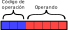
\includegraphics[height=4em]{img/instruccion.pdf}
        \end{figure}

\end{description}

\begin{tabularx}{\textwidth}{c|c|X}

    \textbf{Código de} & \textbf{Operando} &
    \multicolumn{1}{c}{\textbf{Descripción}} \\
    \textbf{operación} & & \\
    \emph{3 bits} & \emph{5 bits} & \\
    \hline
    \hline

    010 & \emph{dirección} & \textbf{Memoria → Acumulador}. Copia un byte
    desde la dirección de memoria al acumulador. \\
    \hline

    011 & \emph{dirección} & \textbf{Acumulador → Memoria}. Copia el contenido
    del acumulador en esa dirección de memoria. \\
    \hline

    100 & \emph{dirección} & \textbf{Suma}. El contenido de la dirección se
    suma al acumulador, y el resultado se almacena en el acumulador. \\
    \hline

    101 & \emph{dirección} & \textbf{Resta}. El contenido de la dirección se
    resta al acumulador, y el resultado se almacena en el acumulador. \\
    \hline

    110 & \emph{desplazamiento} & \textbf{Salto incondicional}. Se suma (en
    complemento a 2) el desplazamiento al \textbf{PC}. \\
    \hline

    111 & \emph{desplazamiento} & \textbf{Salto condicional}. Si el acumulador
    es cero, se suma (en complemento a 2) el desplazamiento al \textbf{PC}, en
    caso contrario el \textbf{PC} se incrementa en uno. \\
    \hline

    001 & \emph{(sin uso)} & \textbf{Detiene la maquina}. No se ejecutan
    nuevas instrucciones. Los registros y la memoria quedan con el último
    valor que tenían. \\
    \hline

    000 & \emph{(sin uso)} & \textbf{No operación}. No tiene ningún efecto
    sobre el acumulador ni memoria. El \textbf{PC} se incremente en uno. \\

\end{tabularx}



\end{document}
